% Vektorgrafiken ausschließlich für die Lesefassung.
% Benötigt nur TikZ ohne zusätzliche Bibliotheken.
\definecolor{bracketingblue}{RGB}{34,92,133}
\definecolor{bracketingshade}{RGB}{226,237,244}

\newcommand{\BracketingTreesDiagram}{%
  \par\medskip\noindent
  \begin{minipage}{\linewidth}
  \centering
  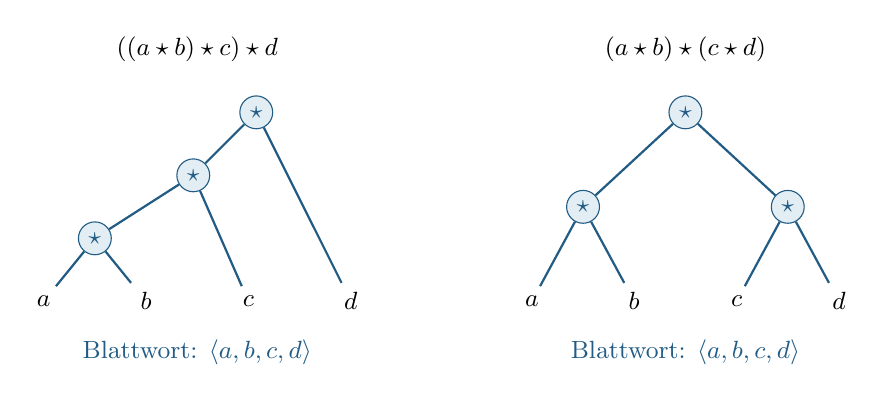
\begin{tikzpicture}[x=1cm,y=1cm,font=\small,
    operation/.style={circle,draw=bracketingblue,fill=bracketingshade,
      inner sep=2pt,text=bracketingblue}]
    \node at (1.95,3.2) {\(((a\star b)\star c)\star d\)};
    \node[operation] (lr) at (2.7,2.4) {\(\star\)};
    \node[operation] (lm) at (1.9,1.6) {\(\star\)};
    \node[operation] (ll) at (.65,.8) {\(\star\)};
    \node (la) at (0,0) {\(a\)};
    \node (lb) at (1.3,0) {\(b\)};
    \node (lc) at (2.6,0) {\(c\)};
    \node (ld) at (3.9,0) {\(d\)};
    \draw[bracketingblue,thick] (lr)--(lm) (lr)--(ld) (lm)--(ll)
      (lm)--(lc) (ll)--(la) (ll)--(lb);

    \node at (8.15,3.2) {\((a\star b)\star(c\star d)\)};
    \node[operation] (rr) at (8.15,2.4) {\(\star\)};
    \node[operation] (rl) at (6.85,1.2) {\(\star\)};
    \node[operation] (rt) at (9.45,1.2) {\(\star\)};
    \node (ra) at (6.2,0) {\(a\)};
    \node (rb) at (7.5,0) {\(b\)};
    \node (rc) at (8.8,0) {\(c\)};
    \node (rd) at (10.1,0) {\(d\)};
    \draw[bracketingblue,thick] (rr)--(rl) (rr)--(rt) (rl)--(ra)
      (rl)--(rb) (rt)--(rc) (rt)--(rd);
    \node[text=bracketingblue] at (1.95,-.65)
      {Blattwort: \(\langle a,b,c,d\rangle\)};
    \node[text=bracketingblue] at (8.15,-.65)
      {Blattwort: \(\langle a,b,c,d\rangle\)};
  \end{tikzpicture}
  \par\smallskip\small\raggedright
  Zwei verschiedene Bäume mit demselben Blattwort. Die Wurzel steht
  oben für die letzte Verknüpfung. Links ist der erste Teilblock
  \(a,b,c\); rechts sind die beiden Teilblöcke \(a,b\) und
  \(c,d\). Ausgewertet wird jeweils von den Blättern zur Wurzel.
  Die Gleichheit der Werte folgt erst aus der Assoziativität und dem Beweis.
  \end{minipage}\par\medskip
}

\newcommand{\BracketingNormalFormDiagram}{%
  \par\medskip\noindent
  \begin{minipage}{\linewidth}
  \centering
  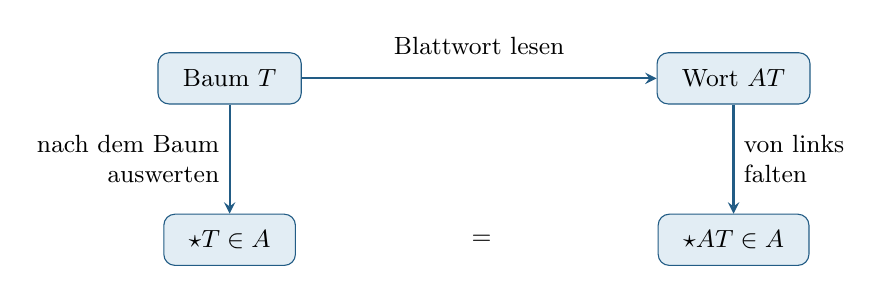
\begin{tikzpicture}[x=1cm,y=1cm,font=\small,>=stealth,
    object/.style={draw=bracketingblue,fill=bracketingshade,
      rounded corners,minimum height=.65cm,inner xsep=9pt}]
    \node[object] (tree) at (0,0) {Baum \(T\)};
    \node[object] (word) at (6.4,0)
      {Wort \(\TreeLeafWord{A}{T}\)};
    \node[object] (value) at (0,-2.05)
      {\(\TreeEvaluation{\star}{T}\in A\)};
    \node[object] (fold) at (6.4,-2.05)
      {\(\WordFold{\star}{\TreeLeafWord{A}{T}}\in A\)};
    \draw[->,thick,bracketingblue] (tree)--
      node[above=5pt,text=black] {Blattwort lesen}(word);
    \draw[->,thick,bracketingblue] (tree)--
      node[left,text=black,align=right] {nach dem Baum\\auswerten}(value);
    \draw[->,thick,bracketingblue] (word)--
      node[right,text=black,align=left] {von links\\falten}(fold);
    \node at (3.2,-2.05) {\(=\)};
  \end{tikzpicture}
  \par\smallskip\small\raggedright
  Die bewiesene Normalform vergleicht zwei Wege zu einem Element von
  \(A\). Links bleibt der ursprüngliche Rechenplan erhalten. Rechts
  werden nur die geordneten Blattbeschriftungen übernommen und mit der
  festen linken Klammerung ausgewertet. In einer Halbgruppe stimmen
  die beiden Ergebnisse überein.
  \end{minipage}\par\medskip
}
